\begin{atiTask}[
  title = Volumenberechnung I,
  %call = Zusatzaufgabe,
]
 Berechnen Sie das von der Fläche
 \begin{equation*}
(x^2+y^2+z^2)^2=a^2(x^2+y^2), \quad a>0
 \end{equation*}
eingeschlossene Volumen. Verwenden Sie dazu Kugelkoordinaten.

\atiNote{Es ist \[\int \sin^4 x\;\D x=\frac{\sin (4 x)-8\sin (2x)+12x}{32}+C\]}
\end{atiTask}
%Lösung Wallner S. 63
\begin{atiSolution}
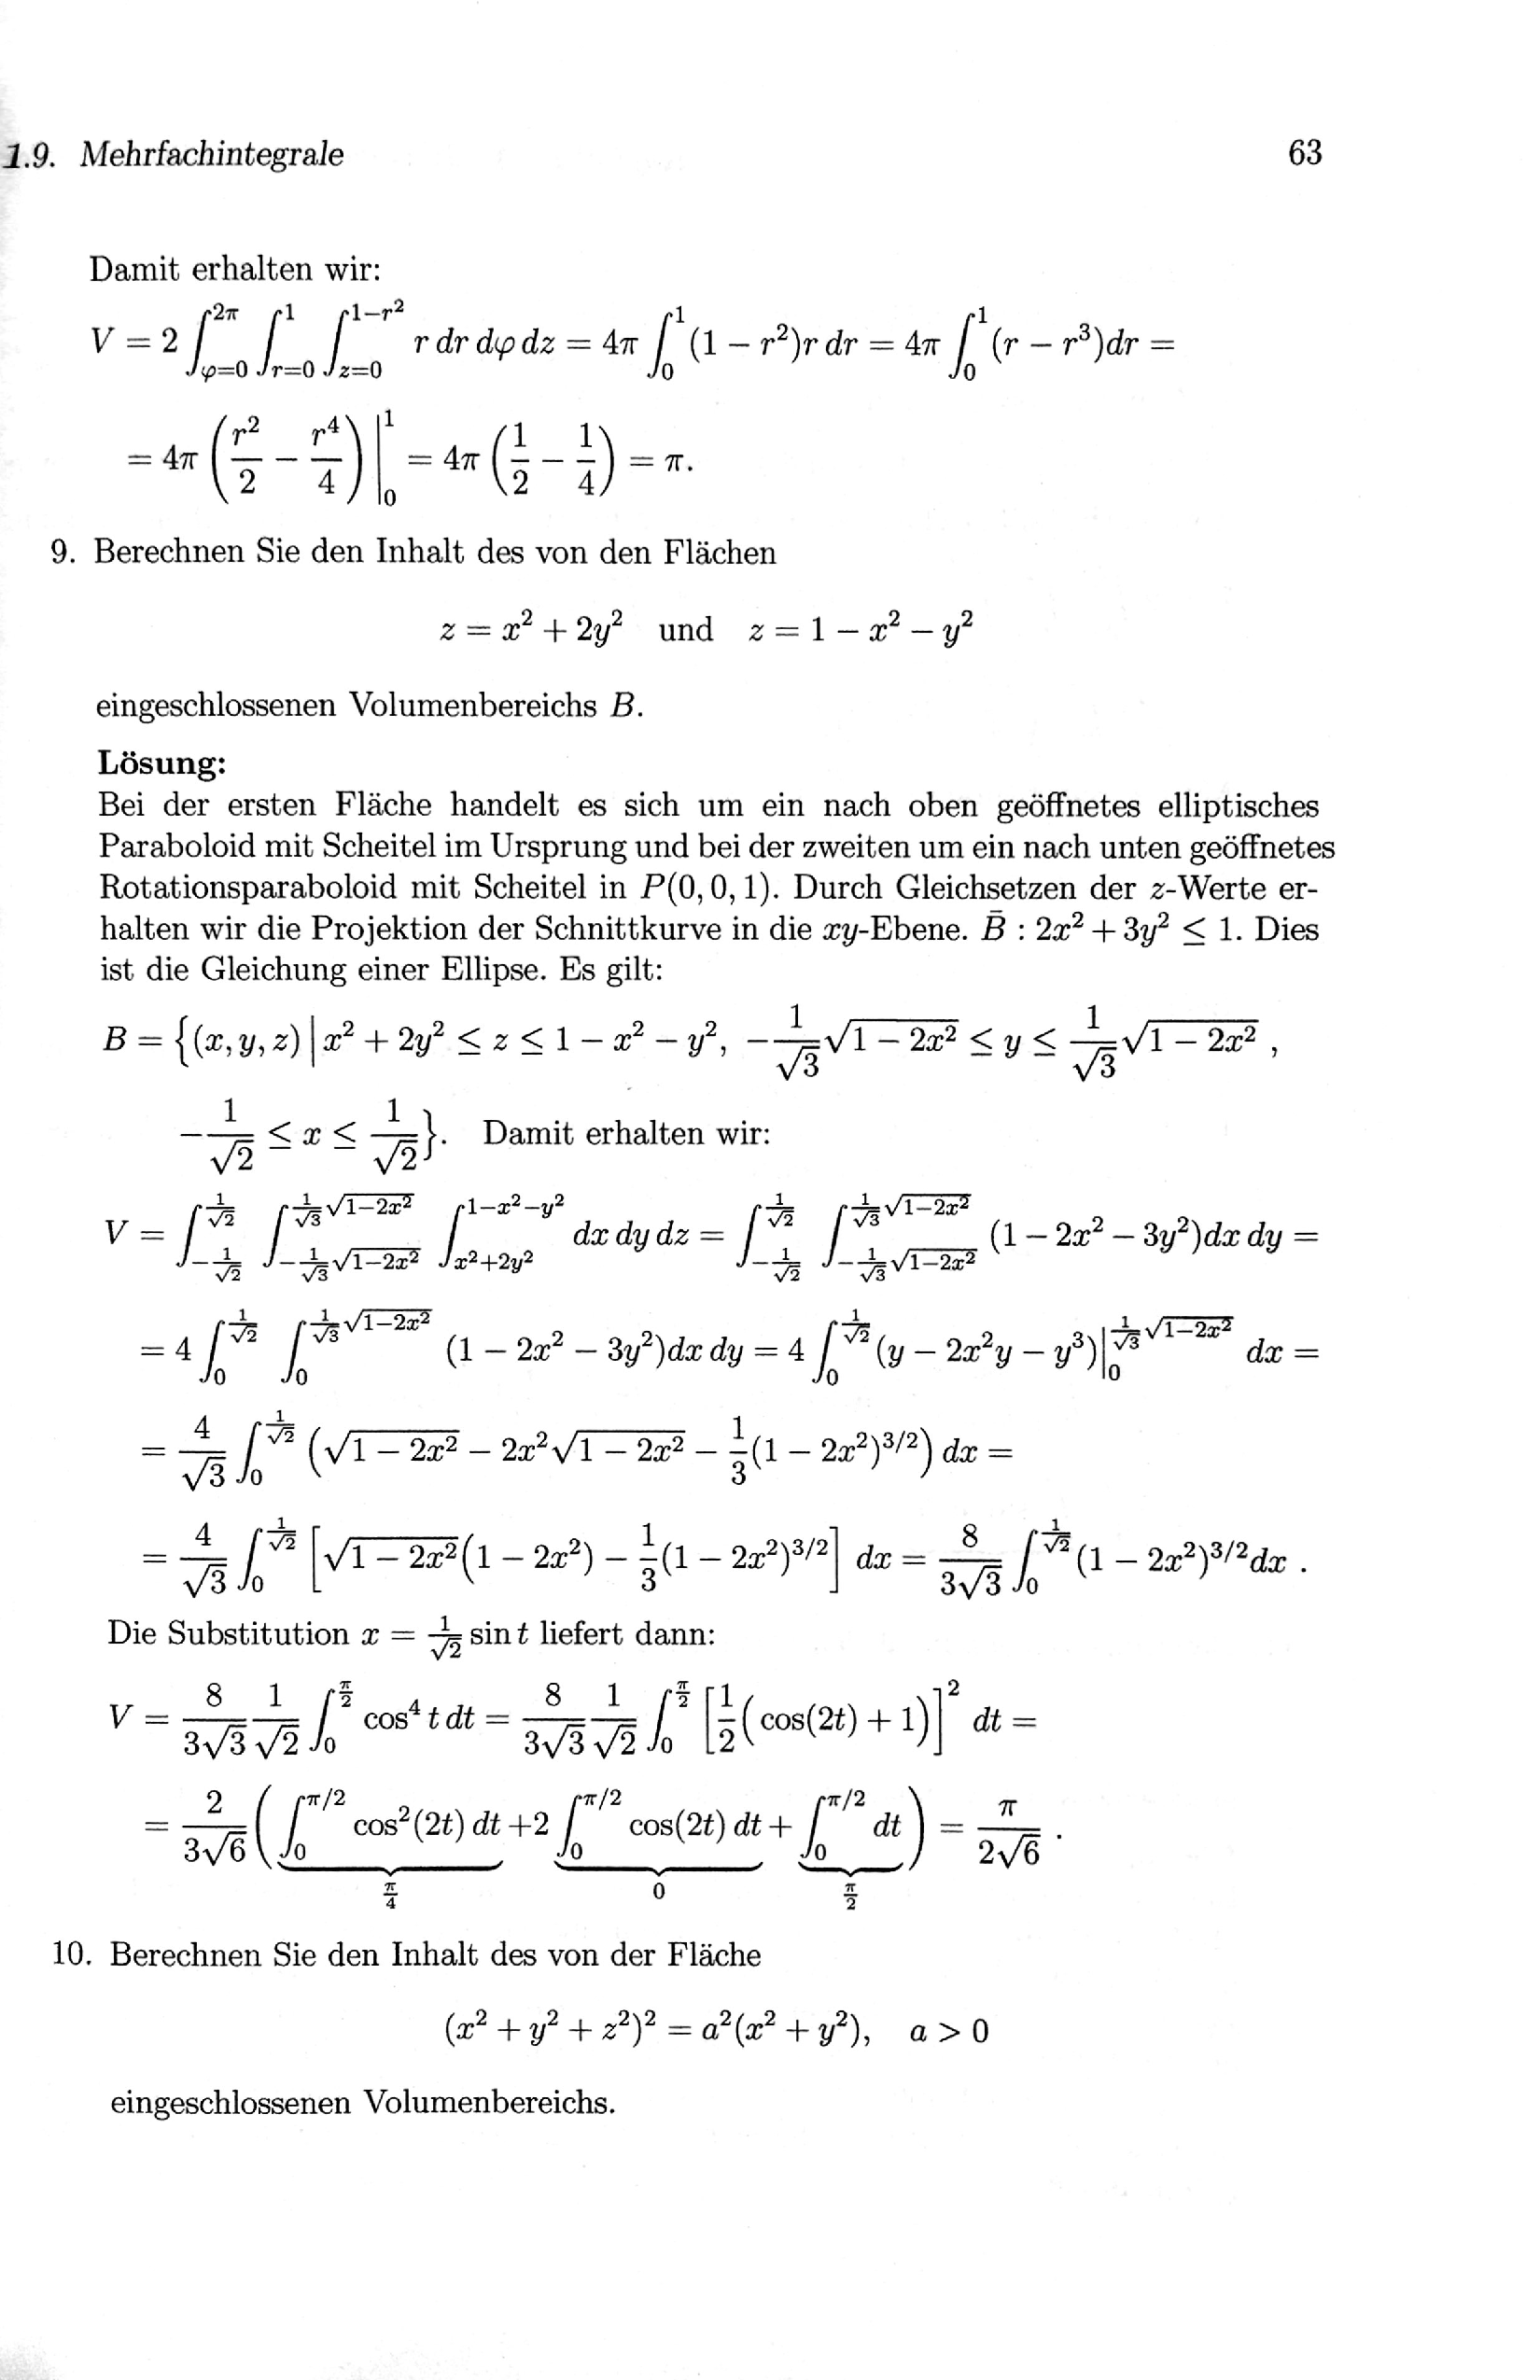
\includepdf[]{solution-dreifachintegral_i.pdf}
\end{atiSolution}
